\section{3D model reconstruction of cloth} \label{section:3dclothrecon}

\subsection{Overview} 

For 3D human body model, we use Skinned Multi-Person Linear model (SMPL)\cite{Loper2015SMPLAS}, because SMPL has well defined control variable for shape and pose and also well defined parameter estimation  algorithms. For similar reasons, SMPL have been utilized in many research works. Furthermore because it is based on blend skinning, SMPL is compatible with existing rendering engines and we make it available for research purposes. SMPL is a skinned vertex-based model that accurately represents a wide variety of body shapes in natural human poses. The parameters of the model are learned from data including the rest pose template, blend weights, pose-dependent blend shapes, identity-dependent blend shapes, and a regressor from vertices to joint locations. Unlike previous models, the pose-dependent blend shapes are a linear function of the elements of the pose rotation matrices. This simple formulation enables training the entire model from a relatively large number of aligned 3D meshes of different people in different poses. \cite{Loper2015SMPLAS} 


\begin{figure}[t]
\centering
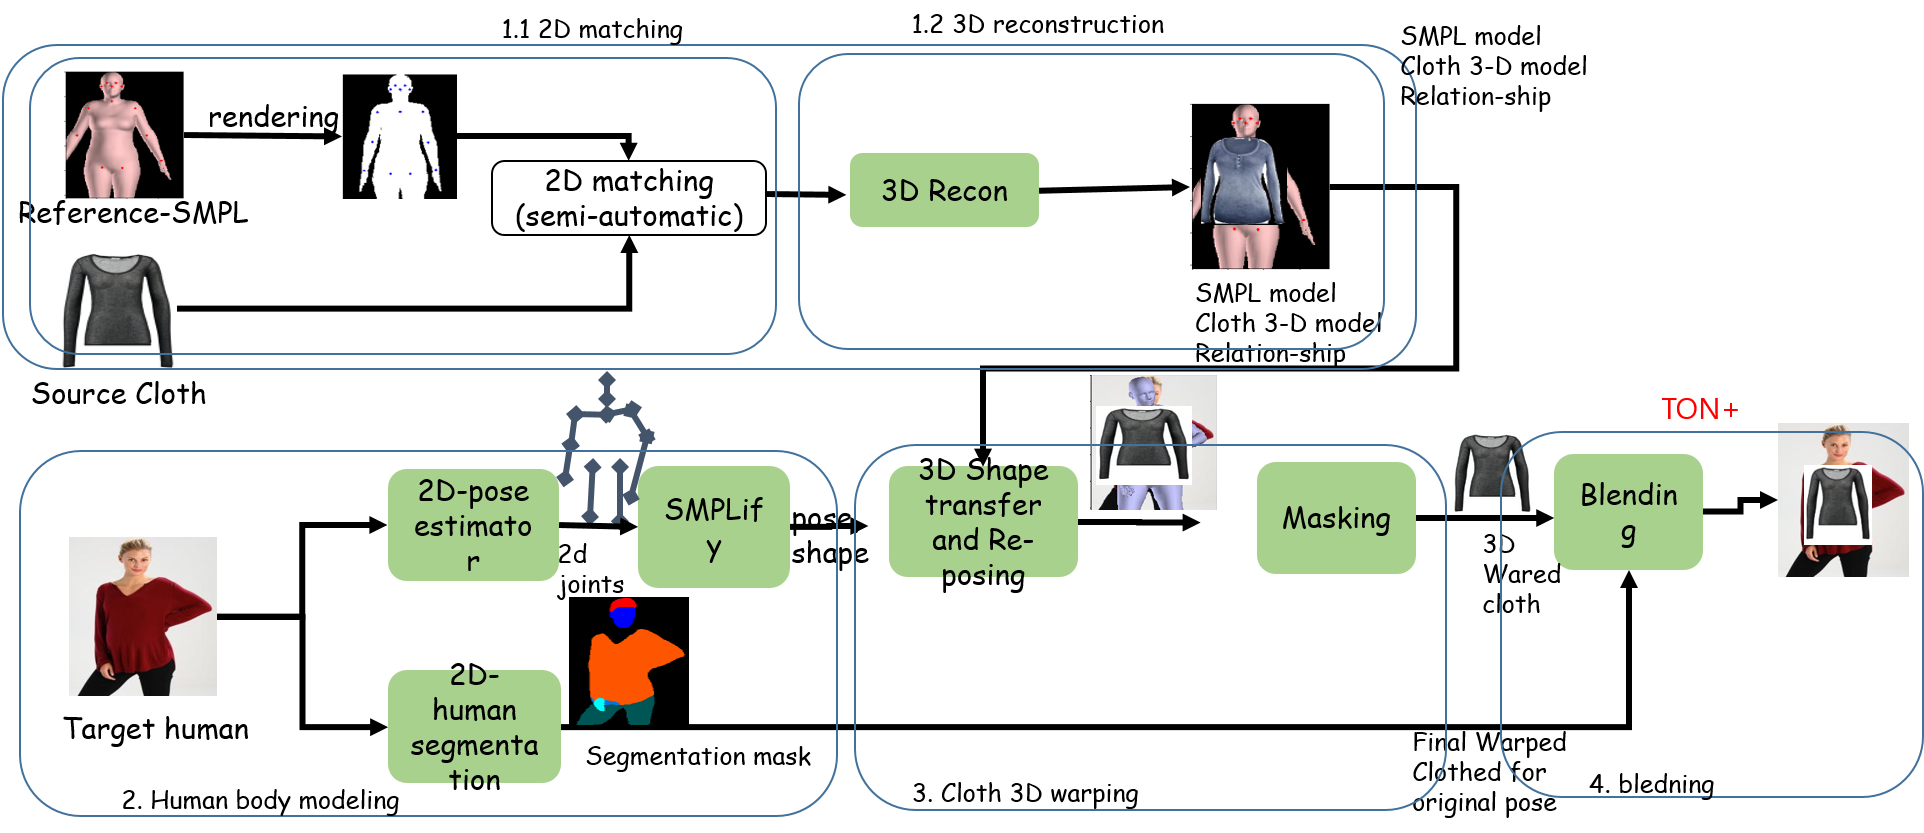
\includegraphics[height=4.5cm, scale=1]{figures/pipeline.png}   % TODO
\caption{Pipeline}
\label{fig:piepline}
\end{figure}


For estimating the SMPL parameters, we use SMPLify\cite{Bogo2016SMPLify} method in this study. However any other methods can be used because we assume nothing on the procedure and use estimated parameters only. SMPLify uses 2D human body joint information often obtained from deep learning based method like DeepCut or OpenPose, and minimize the projected joint locations and the given (considered true) 2D joint locations. The cost function can include other priors and silhouette information. We made minor optimization for half body dataset, such as joint location mapping between the joints of used fashion data set and SMPLify joint definition, and conditional inclusion of invisible joints and initialization step.  From our experiments with all 2032 test images, we found that the SMPLify quality should be much improved for fully automatic application to VTON application. So the result included in this paper excluded the bad matching cases which is around 30\% of all test images.    
  
Clothed human reconstruction using SMPL have been studied in several previous works \cite{Weng2018PhotoW3,Zanfir2018HumanAT}.
Even we are successful in modeling human body, there are further difficulty to recover the clothed human model from body model. It is because the cloth vertices are not directly corresponds to the human body's, and even though it has it is still difficult to estimate the difference between two. Also the texture of cloth can be occluded by other part of cloth and human body parts. The previous work try to solve the problem in the given image condition. Therefore the results are strongly dependent upon the input image.
In this paper, we make this step easy using simple standard human pose, where all frontal part of cloth is well separated and visible. This setup cannot handle all problem in the clothed human model reconstruction but can greatly make it easy.   
The following subsection describe the procedure in details.



\subsection{2D Standard Cloth matching}


To align the try-on cloth image with 3D SMPL body model\cite{Loper2015SMPLAS}, first their dimension spaces should be matched. Natural way would be first rendering the SMPL body model into 2D image space. However, again the matching with cloth image and body silhouette is not a simple task, for simplicity we assume we can segment the silhouette so that the the remaining area can be easily matched by SCM algorithms. We argue that this step can be monitored by service provider which is practically acceptable; the manual operation from the customer in the try-on step would be not acceptable in general service environment.   

\begin{equation}
(I_{c, warped}, M_{c, warped})  = T_{SMPL} ((I_c, M_c))
\end{equation}


\begin{figure}[t]
\centering
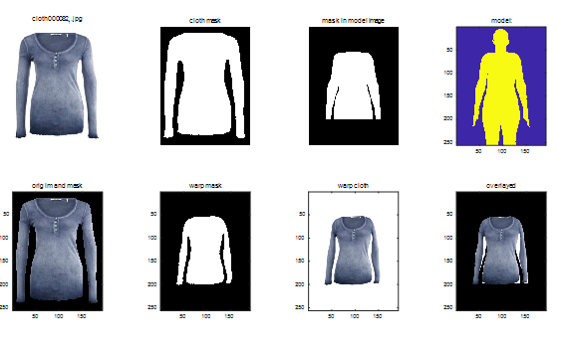
\includegraphics[height=6.5cm, scale=0.7]{figures/2dmatching.png}   % TODO
\caption{2D Matching}
\label{fig:2DmatchingOfClothAndBody}
\end{figure}


\subsection{3D cloth model reconstruction }


The 3D reconstruction process from aligned cloth image and projected silhouette consists of 2 steps. First, the vertices of 3D body mesh are projected into 2D image space, the boundary  vertices in 2D spaces and the cloth boundaries are used for corresponding points. The corresponding points in the cloth boundary i defined the closest points from the projected vertices.  This step works well in our cases differently from PhotoWakeup study, because the part of body and cloth are not self-overlapped. This is a implementation benefits of our approach. From the corresponding point pairs, a TPS paramter are estimated and applied to the mesh points. The new mesh points are considered the vertices projected from 3D mesh of cloth.    

From the 2D points to 3D points are done with inverse projection with depth obtained from the body with a small constant gap. In reality the gap between the cloth and body cannot be constant but it works with tight or simple clothes. Further research should be needed for accurate depth estimation.   

\begin{equation}
V_{clothed} = Pjt^{-1} ( T( (Pjt(V_{body})), depth(V_{body}) )
\end{equation}


The try-on cloth images are used for the texture for the 3D cloth mesh. We can filter the vertices corresponding to cloth and get the cloth 3D mesh model. Figure xxxxx shows the reconstructed cloth examples. 


Discussions needed


\begin{figure}[t]
\centering
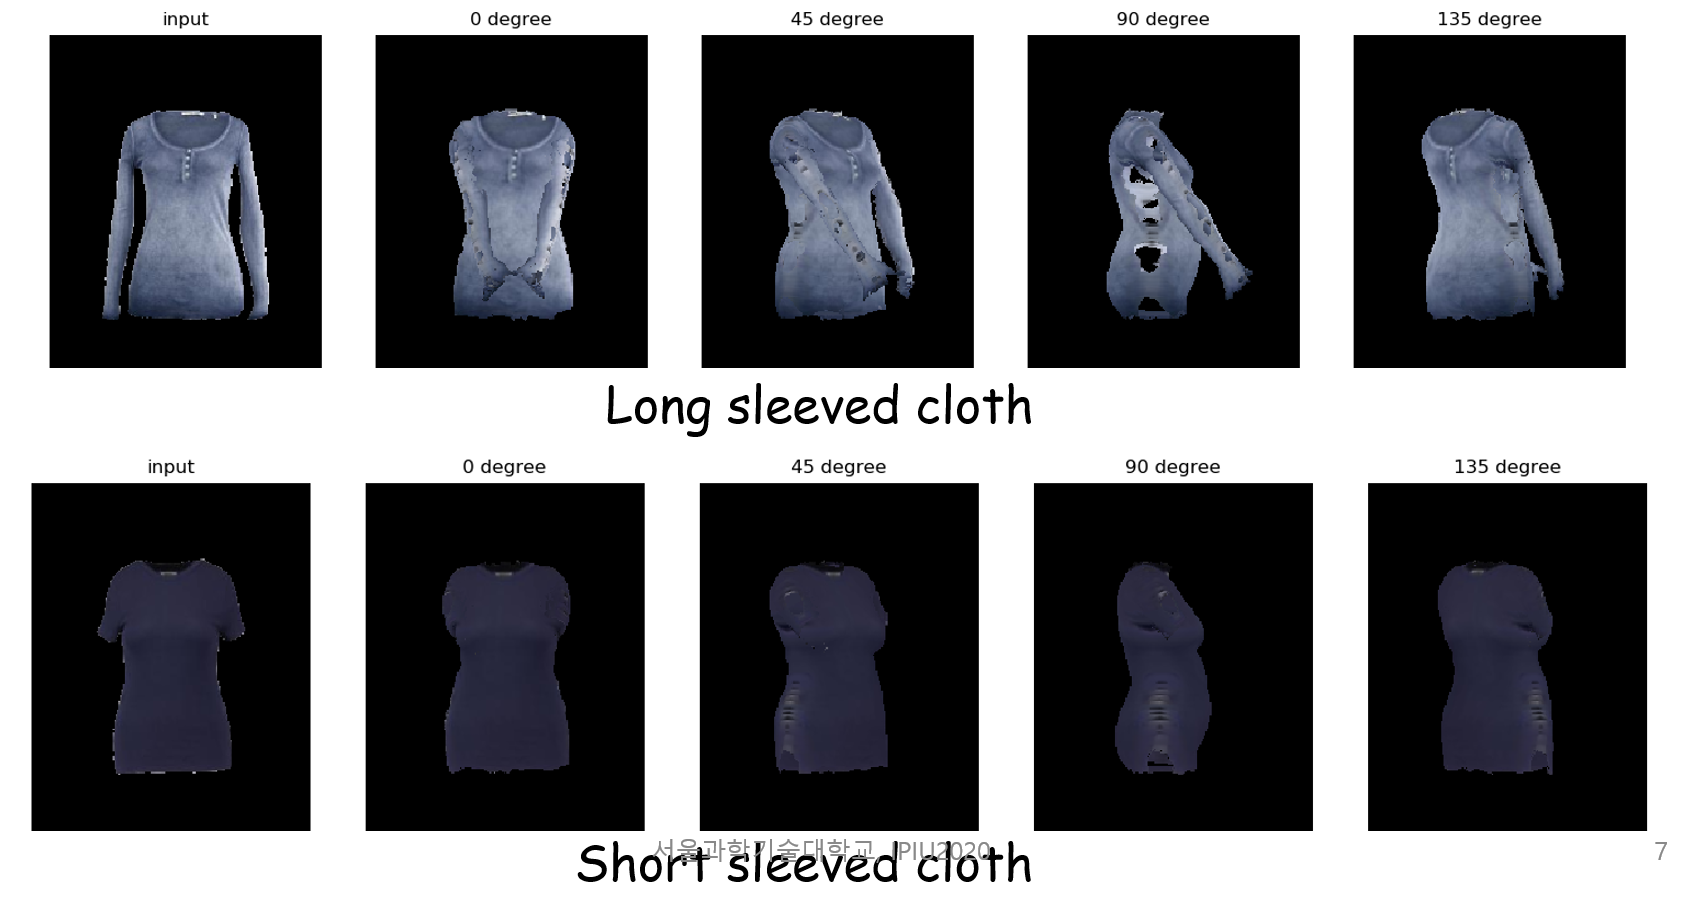
\includegraphics[height=6.5cm, scale=1]{figures/3dclothrecon.png}   % TODO
\caption{3D reconstructed cloth}
\label{fig:3DreconstructedCloth}
\end{figure}



